\documentclass[mathserif,compress]{beamer}

\mode<presentation>
{
  \usecolortheme{orchid}
  \useoutertheme{shadow}
}
\newcommand\hmmax{0}
\newcommand\bmmax{0}
\usepackage{natbib, verbatim}

\usepackage[utf8]{inputenc}

\usepackage{mathpazo}
\usepackage[T1]{fontenc}

\usepackage{amsmath}
\usepackage{amsthm}
\usepackage{amssymb}
\usepackage{mathptmx}
\usepackage{anyfontsize}
\usepackage{t1enc}
\usepackage{appendix}
\usepackage{array}
\usepackage{bm}
\usepackage{cancel}
\usepackage{cite}
\usepackage{courier}
\usepackage{graphicx}
\usepackage{empheq}
\usepackage{enumerate}
\usepackage{listings}
\usepackage{mathtools}
\usepackage{units}
\usepackage{bigstrut}
\usepackage{rotating}
\usepackage{ mathrsfs }
\usepackage{multirow}
\usepackage{booktabs}
\usepackage{algorithm, algorithmic}

\DeclareMathAlphabet{\mathcal}{OMS}{cmsy}{m}{n}

\DeclareMathAlphabet{\mathsfit}{\encodingdefault}{\sfdefault}{m}{}
\SetMathAlphabet{\mathsfit}{bold}{\encodingdefault}{\sfdefault}{bx}{}

\newcommand{\tens}[1]{\bm{\mathsfit{#1}}}

\usepackage{color}
\lstset{language=R,basicstyle=\ttfamily,breaklines=true,
                keywordstyle=\color{blue}\ttfamily,
                stringstyle=\color{red}\ttfamily,
                commentstyle=\color{magenta}\ttfamily,
                showstringspaces=false,
                }

\newcommand*\widefbox[1]{\fbox{\hspace{2em}#1\hspace{2em}}}
\newcommand*\mb{\mathbf}
\newcommand*\reals{\mathbb{R}}
\newcommand*\complex{\mathbb{C}}
\newcommand*\naturals{\mathbb{N}}
\newcommand*\nats{\naturals}
\newcommand*\integers{\mathbb{Z}}
\newcommand*\rationals{\mathbb{Q}}
\newcommand*\irrationals{\mathbb{J}}
\newcommand*\pd{\partial}
\newcommand*\htab{\hspace{4 mm}}
\newcommand*\vtab{\vspace{0.5 in}}
\newcommand*\lsent{\mathcal{L}}
\newcommand*\conj{\overline}
\newcommand*\union{\cup}
\newcommand*\intersect{\cap}
\newcommand*\cl{\cancel}
\newcommand*\ANS{\text{ANS}}
\newcommand*\As{\text{As}}
\newcommand*\then{\rightarrow}
\newcommand*\elim{\text{E}}
\newcommand*\intro{\text{I}}
\newcommand*\absurd{\curlywedge}
\newcommand*\NK{\vdash_{\text{NK}}}
\newcommand*\derivation{\begin{tabular} { >{$}l<{$}  >{$}c<{$}  >{$}l<{$}  >{$}r<{$} }}
\newcommand*\interp{\mathcal{I}}
\newcommand*\ba{\[ \begin{aligned}}
\newcommand*\ea{\end{aligned} \]}
\newcommand*\C{\mathcal{C}}
\newcommand*\D{\mathscr{D}}
\newcommand*\e{\operatorname{e}}
\newcommand*\df{=_{\text{def}}}
\newcommand*\eps{\epsilon}
\newcommand*\enum{\begin{enumerate}[label=(\alph*)]}
\newcommand*\enumend{\end{enumerate}}
\newcommand*\E[1]{\tens{E}\left[#1\right]}
\newcommand*\Esub[2]{\mathsf{E}_{#1}\left[#2\right]}
\newcommand*\Var[1]{\tens{Var}\left[#1\right]}
\newcommand*\Cov[1]{\tens{Cov}\left[#1\right]}
\newcommand*\iid{\overset{\text{iid}}{\sim}}
\newcommand*\Exp[1][\lambda]{\text{Exp}(\text{rate}=#1)}
\newcommand*\ind[2]{I_{({#1}, {#2})} }
\newcommand*\set[1]{\left\{#1\right\}}
\newcommand*\estim[1]{\widehat{#1}}
\newcommand*\der{\text{d}}
\newcommand*\norm[1]{\left\|#1\right\|}
\newcommand*\dist[2]{\;\text{dist}\left(#1, #2\right)}
\newcommand*\interior{\text{int}\;}
\newcommand*\exterior{\text{ext}\;}
\newcommand*\boundary{\text{bd}\;}
\newcommand*\lh{\overset{\text{L'H}}{=}}

\renewcommand\Re{\operatorname{Re}}
\renewcommand\Im{\operatorname{Im}}
\DeclareMathOperator*{\argmin}{arg\;min}
\renewcommand\;{\,}
\renewcommand\epsilon{\varepsilon}
\renewcommand\rho{\varrho}
\renewcommand\phi{\varphi}
\renewcommand\mod{\hspace{0.2em} \textbf{mod}\hspace{0.2em}}
\renewcommand\Pr[1]{ \tens{Pr}\left[#1\right] }
\def\ci{\perp\!\!\!\perp}

\usepackage{tikz}
\usetikzlibrary{positioning}
\usetikzlibrary{shapes,arrows}
\usepackage{adjustbox}

\tikzstyle{decision} = [diamond, draw, fill=blue!20, 
    text width=4.5em, text badly centered, node distance=3cm, inner sep=0pt]
\tikzstyle{block} = [rectangle, draw, fill=blue!20, 
    text width=6em, text centered, rounded corners, minimum height=4em]
\tikzstyle{line} = [draw, -latex']
\tikzstyle{cloud} = [draw, ellipse,fill=red!20, node distance=3cm,
    minimum height=2em]

\lstset{breaklines=true,
        numbersep=5pt,
        xleftmargin=.25in,
        xrightmargin=.25in}

\DeclareMathOperator{\sech}{sech}
\DeclareMathOperator{\sgn}{sgn}
\makeatletter
\renewcommand*\env@matrix[1][*\c@MaxMatrixCols c]{%
  \hskip -\arraycolsep
  \let\@ifnextchar\new@ifnextchar
  \array{#1}}
\makeatother

\newenvironment{amatrix}[1]{%
  \left(\begin{array}{@{}*{#1}{c}|c@{}}
}{%
  \end{array}\right)
}

\lstset{basicstyle=\footnotesize\ttfamily,breaklines=true}


\newcommand{\real}{\ensuremath{\mathbb{R}}}
\newcommand{\bA}{\mbox{\protect\boldmath $A$}}
\newcommand{\bo}{\mbox{\protect\boldmath $o$}}
\newcommand{\bu}{\mbox{\protect\boldmath $u$}}
\newcommand{\by}{\mbox{\protect\boldmath $y$}}
\newcommand{\bx}{\mbox{\protect\boldmath $x$}}
\newcommand{\bs}{\mbox{\protect\boldmath $s$}}
\newcommand{\bS}{\mbox{\protect\boldmath $S$}}
\newcommand{\bz}{\mbox{\protect\boldmath $z$}}
\newcommand{\bh}{\mbox{\protect\boldmath $h$}}
\newcommand{\bF}{\mbox{\protect\boldmath $f$}}
\newcommand{\bt}{\mbox{\protect\boldmath $t$}}
\newcommand{\bc}{\mbox{\protect\boldmath $c$}}
\newcommand{\bC}{\mbox{\protect\boldmath $C$}}
\newcommand{\bV}{\mbox{\protect\boldmath $V$}}
\newcommand{\bX}{\mbox{\protect\boldmath $X$}}
\newcommand{\bW}{\mbox{\protect\boldmath $W$}}
\newcommand{\bZ}{\mbox{\protect\boldmath $Z$}}
\newcommand{\bof}{\mbox{\protect\boldmath $f$}}
\newcommand{\indicator}{{\ensuremath{\mathbb{I}}}}
\newcommand{\M}{{\ensuremath{\rm M}}}
\newcommand{\bbeta}{\boldsymbol{\beta}}
\newcommand{\balpha}{\boldsymbol{\alpha}}
\newcommand{\bgamma}{\boldsymbol{\gamma}}
\newcommand{\bdelta}{\boldsymbol{\delta}}
\newcommand{\btheta}{\boldsymbol{\theta}}
\newcommand{\bzero}{\mathbf{0}}
\newcommand{\hsp}{\hspace{0.2mm}}

\footnotesize

\beamertemplatenavigationsymbolsempty
\setbeamertemplate{headline}{\vskip2pt}

\title[]{Immune receptor repertoire summaries and comparison via \texttt{sumrep}}

\author[]
{Branden Olson, Erick Matsen, and lots of AIRR software-wg folks}

\date[Sept. 24, 2018]
{September 24, 2018}

\institute[]
{
Fred Hutch
}

\AtBeginSection[]
{
   \begin{frame}
       \frametitle{Outline}
       \tableofcontents[currentsection]
   \end{frame}
}

\begin{document}

\begin{frame}[noframenumbering]
  \titlepage
\end{frame}

\section{Repertoire summaries and comparisons}

\begin{frame}\frametitle{The formation of BCRs (TCRs are simpler)}
\begin{center}
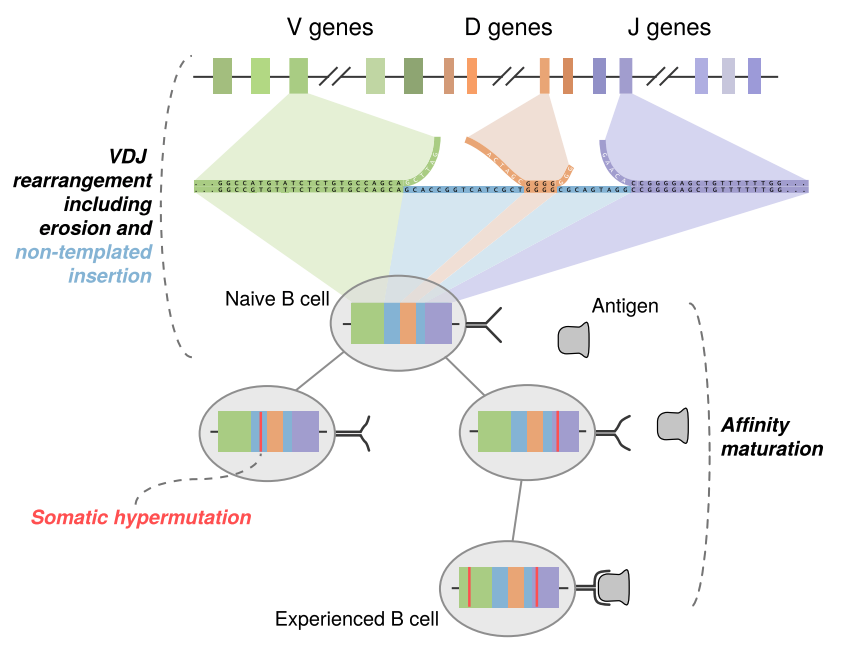
\includegraphics[width=\linewidth]{Images/BCRFormation.png}
\end{center}
\end{frame}

\begin{frame}\frametitle{Motivation}
Immune repertoire sequence datasets are large and complex:
\begin{center}
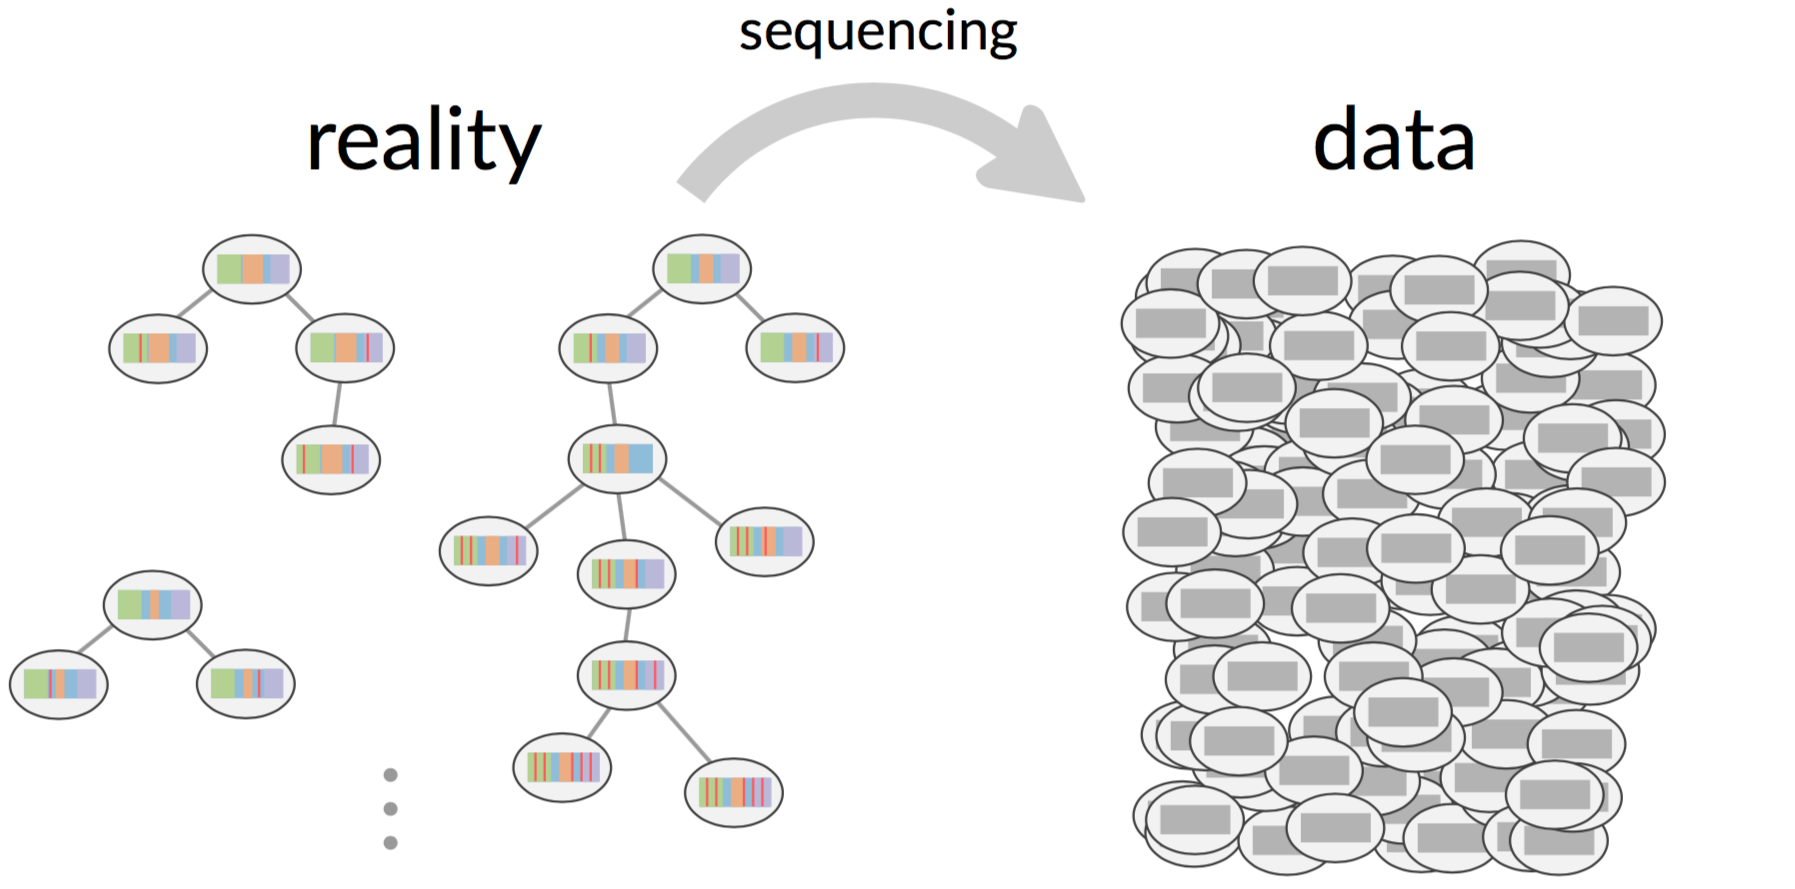
\includegraphics[width=\linewidth]{Images/reality-data.png}
\end{center}
$\implies$ How should we characterize them?
\end{frame}

\begin{frame}\frametitle{Goals}
\begin{itemize}
\item
Idea: Summary statistics reduce a repertoire to comparable quantities
\bigskip
\item
Goal: Build a comprehensive framework for repertoire characterization and comparison via \emph{lots} of summary statistics
\bigskip
\item
Goal (in progress): Evaluate the statistics (e.g. robustness to noise, orthogonality) 
\bigskip
\item
Application (in progress): Generative model validation
\end{itemize}
\end{frame}

\begin{frame}\frametitle{Coming up with summaries}
\begin{itemize}
\item
Teamed up with many scientists in the Adaptive Immune Receptor Repertoire (AIRR) community:
\bigskip
\item[]
\begin{center}
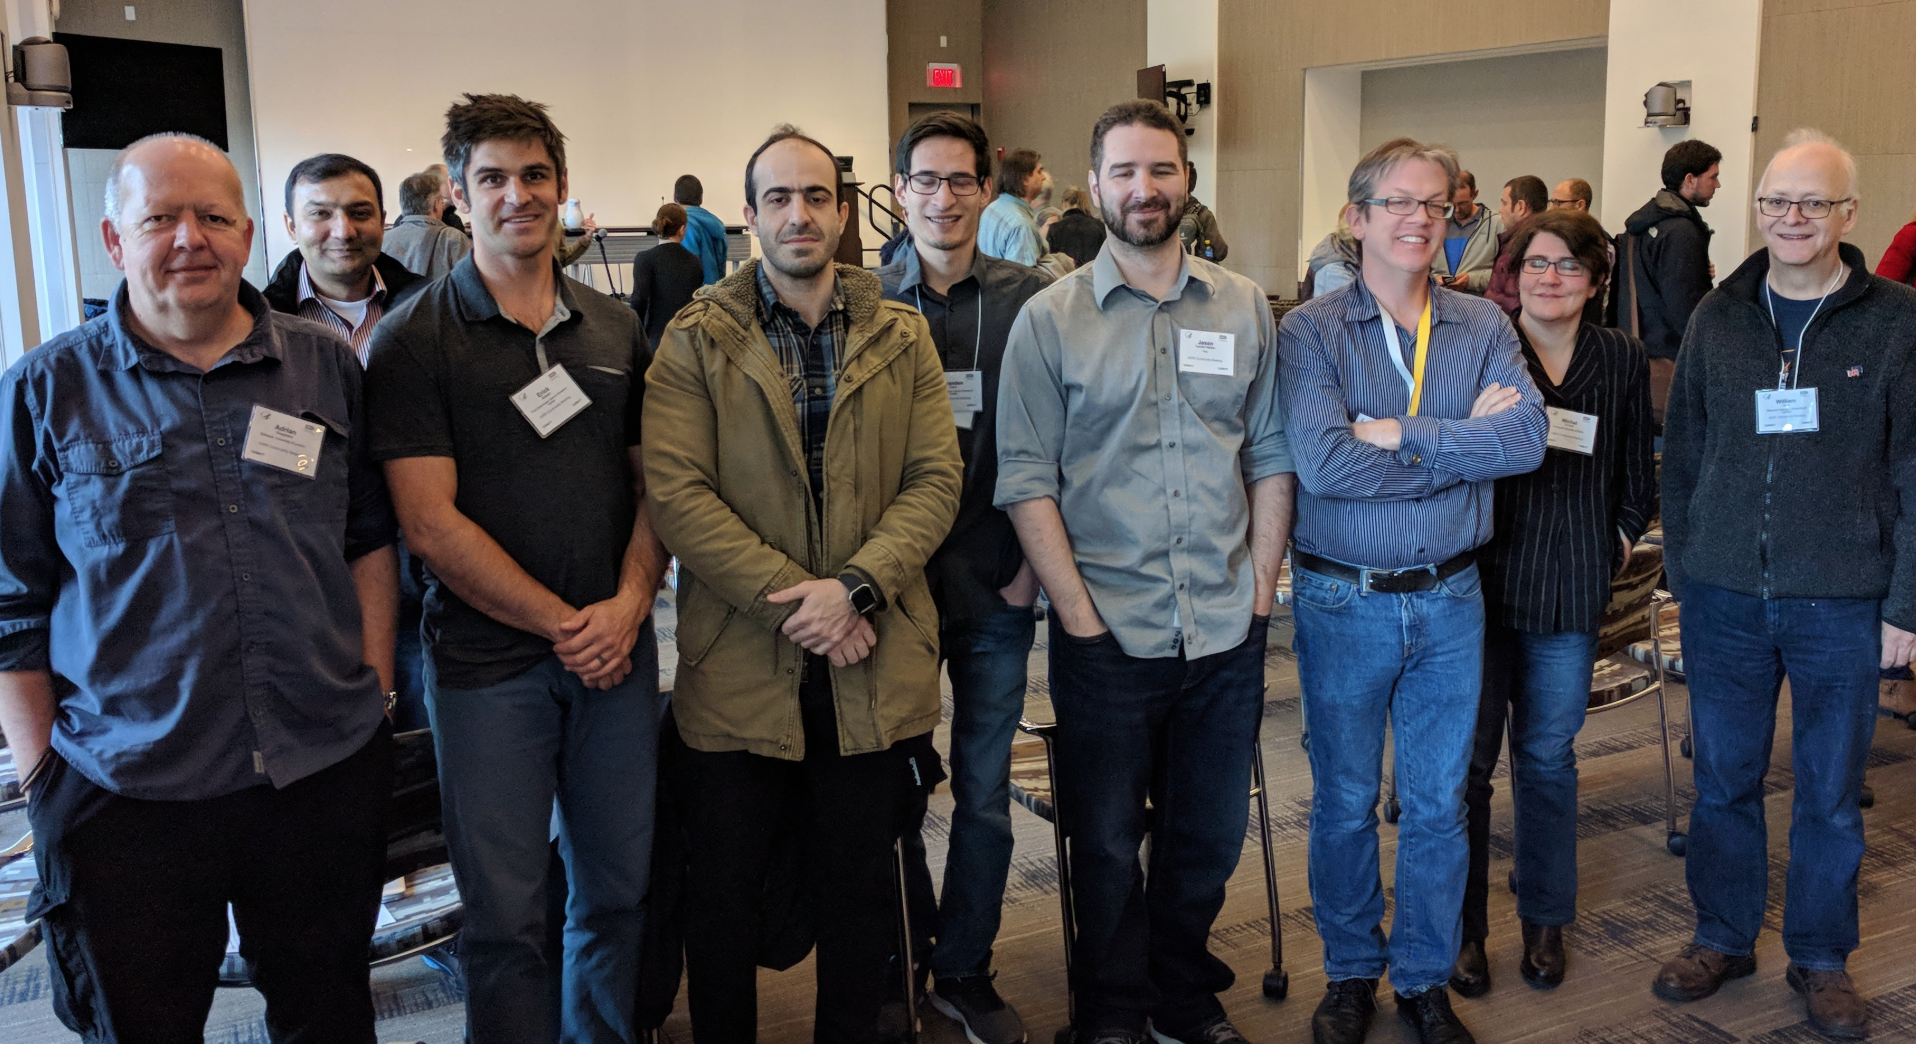
\includegraphics[width=0.9\linewidth]{Images/AIRR.png}
\end{center}
\bigskip
\item
Came up with many stats, from simple DNA stats to specific, complex B/TCR summaries
\end{itemize}
\end{frame}

\begin{frame}\frametitle{Current table of (38) statistics}
\fontsize{5}{7.5}\selectfont
\begin{tabular}{c|c|c|c|c}
    Summary statistic & Annotations & Clustering & Phylogeny & Implementation
\\
\hline \hline
Pairwise distance distribution & No & No & No & \texttt{stringdist} \\
$k$th nearest neighbor distribution & No & No & No & \texttt{stringdist} \\
GC-content distribution & No & No & No & \texttt{ape} \\
Hot/cold spot motif count distribution & No & No & No & \texttt{Biostrings} \\
%BJO Hmm... we never really did much with this (i.e. the Eulerian path paper). Maybe we should discuss?
$k$mer frequency & No & No & No & TBD \\
\hline
Distance from naive to mature distribution & Yes & No & No & \texttt{stringdist} \\
%BJO Another one we kind of skipped over.
$k$th nearest neighbor (V-sequence) distribution & Yes & No & No &\texttt{stringdist},  \texttt{sumrep} \\
CDR3 length distribution & Yes & No & No & Tool-provided \\
Joint distribution of germline gene use & Yes & No & No & \texttt{sumrep} \\
Pairwise CDR3 distance distribution & Yes & No & No & \texttt{stringdist} \\
Hydrophobicity distribution & Yes & No & No & \texttt{Peptides} \\
Atchley factors distribution & Yes & No & No & \texttt{HDMD} \\
Aliphatic index distribution & Yes & No & No & \texttt{Peptides} \\
G.R.A.V.Y. index distribution & Yes & No & No & \texttt{alakazam} \\
Per-gene substitution rate & Yes & No & No & Tool-provided + \texttt{sumrep} \\
Per-gene-per-position substitution rate & Yes & No & No & Tool-provided + \texttt{sumrep} \\
Per-base mutability model & Yes & No & No & \texttt{shazam} \\
Per-base substitution model & Yes & No & No & \texttt{shazam} \\
%BJO This one doesn't depend on fit-star, right?
%EM Yes, but we could just count Ts vs Tv, call it a "ratio" and drop the model-based rigor.
Transition/transversion ratio distribution & Yes & No & No & \texttt{sumrep} \\
Positional distance between mutations distribution & Yes & No & No & \texttt{sumrep}  \\
Distance from naive to mature distribution & Yes & No & No & \texttt{stringdist} \\
V/D/J deletion/insertion lengths distribution & Yes & No & No & Tool-provided \\
Transition matrix for insertions & Yes & No & No & \texttt{sumrep} \\
\hline
Cluster size distribution & Yes & Yes & No & Custom \\
Hill numbers (diversity indices) & Yes & Yes & No & \texttt{alakazam} \\
Selection estimates & Yes & Yes & No & \texttt{shazam} \\
%BJO blocked due to fit-star
Transition/transversion rates & Yes & Yes & No & Tool-provided \\
\hline
Sackin index distribution & Yes & Yes & Yes & \texttt{CollessLike} \\
Colless-like index distribution & Yes & Yes & Yes & \texttt{CollessLike} \\
Cophenetic index distribution & Yes & Yes & Yes & \texttt{CollessLike} \\
%BJO To be delineated
Graph-theoretical features & Yes & Yes & Yes & TBD \\
\end{tabular}
\end{frame}

\begin{frame}\frametitle{Univariate distribution plots}
\begin{center}
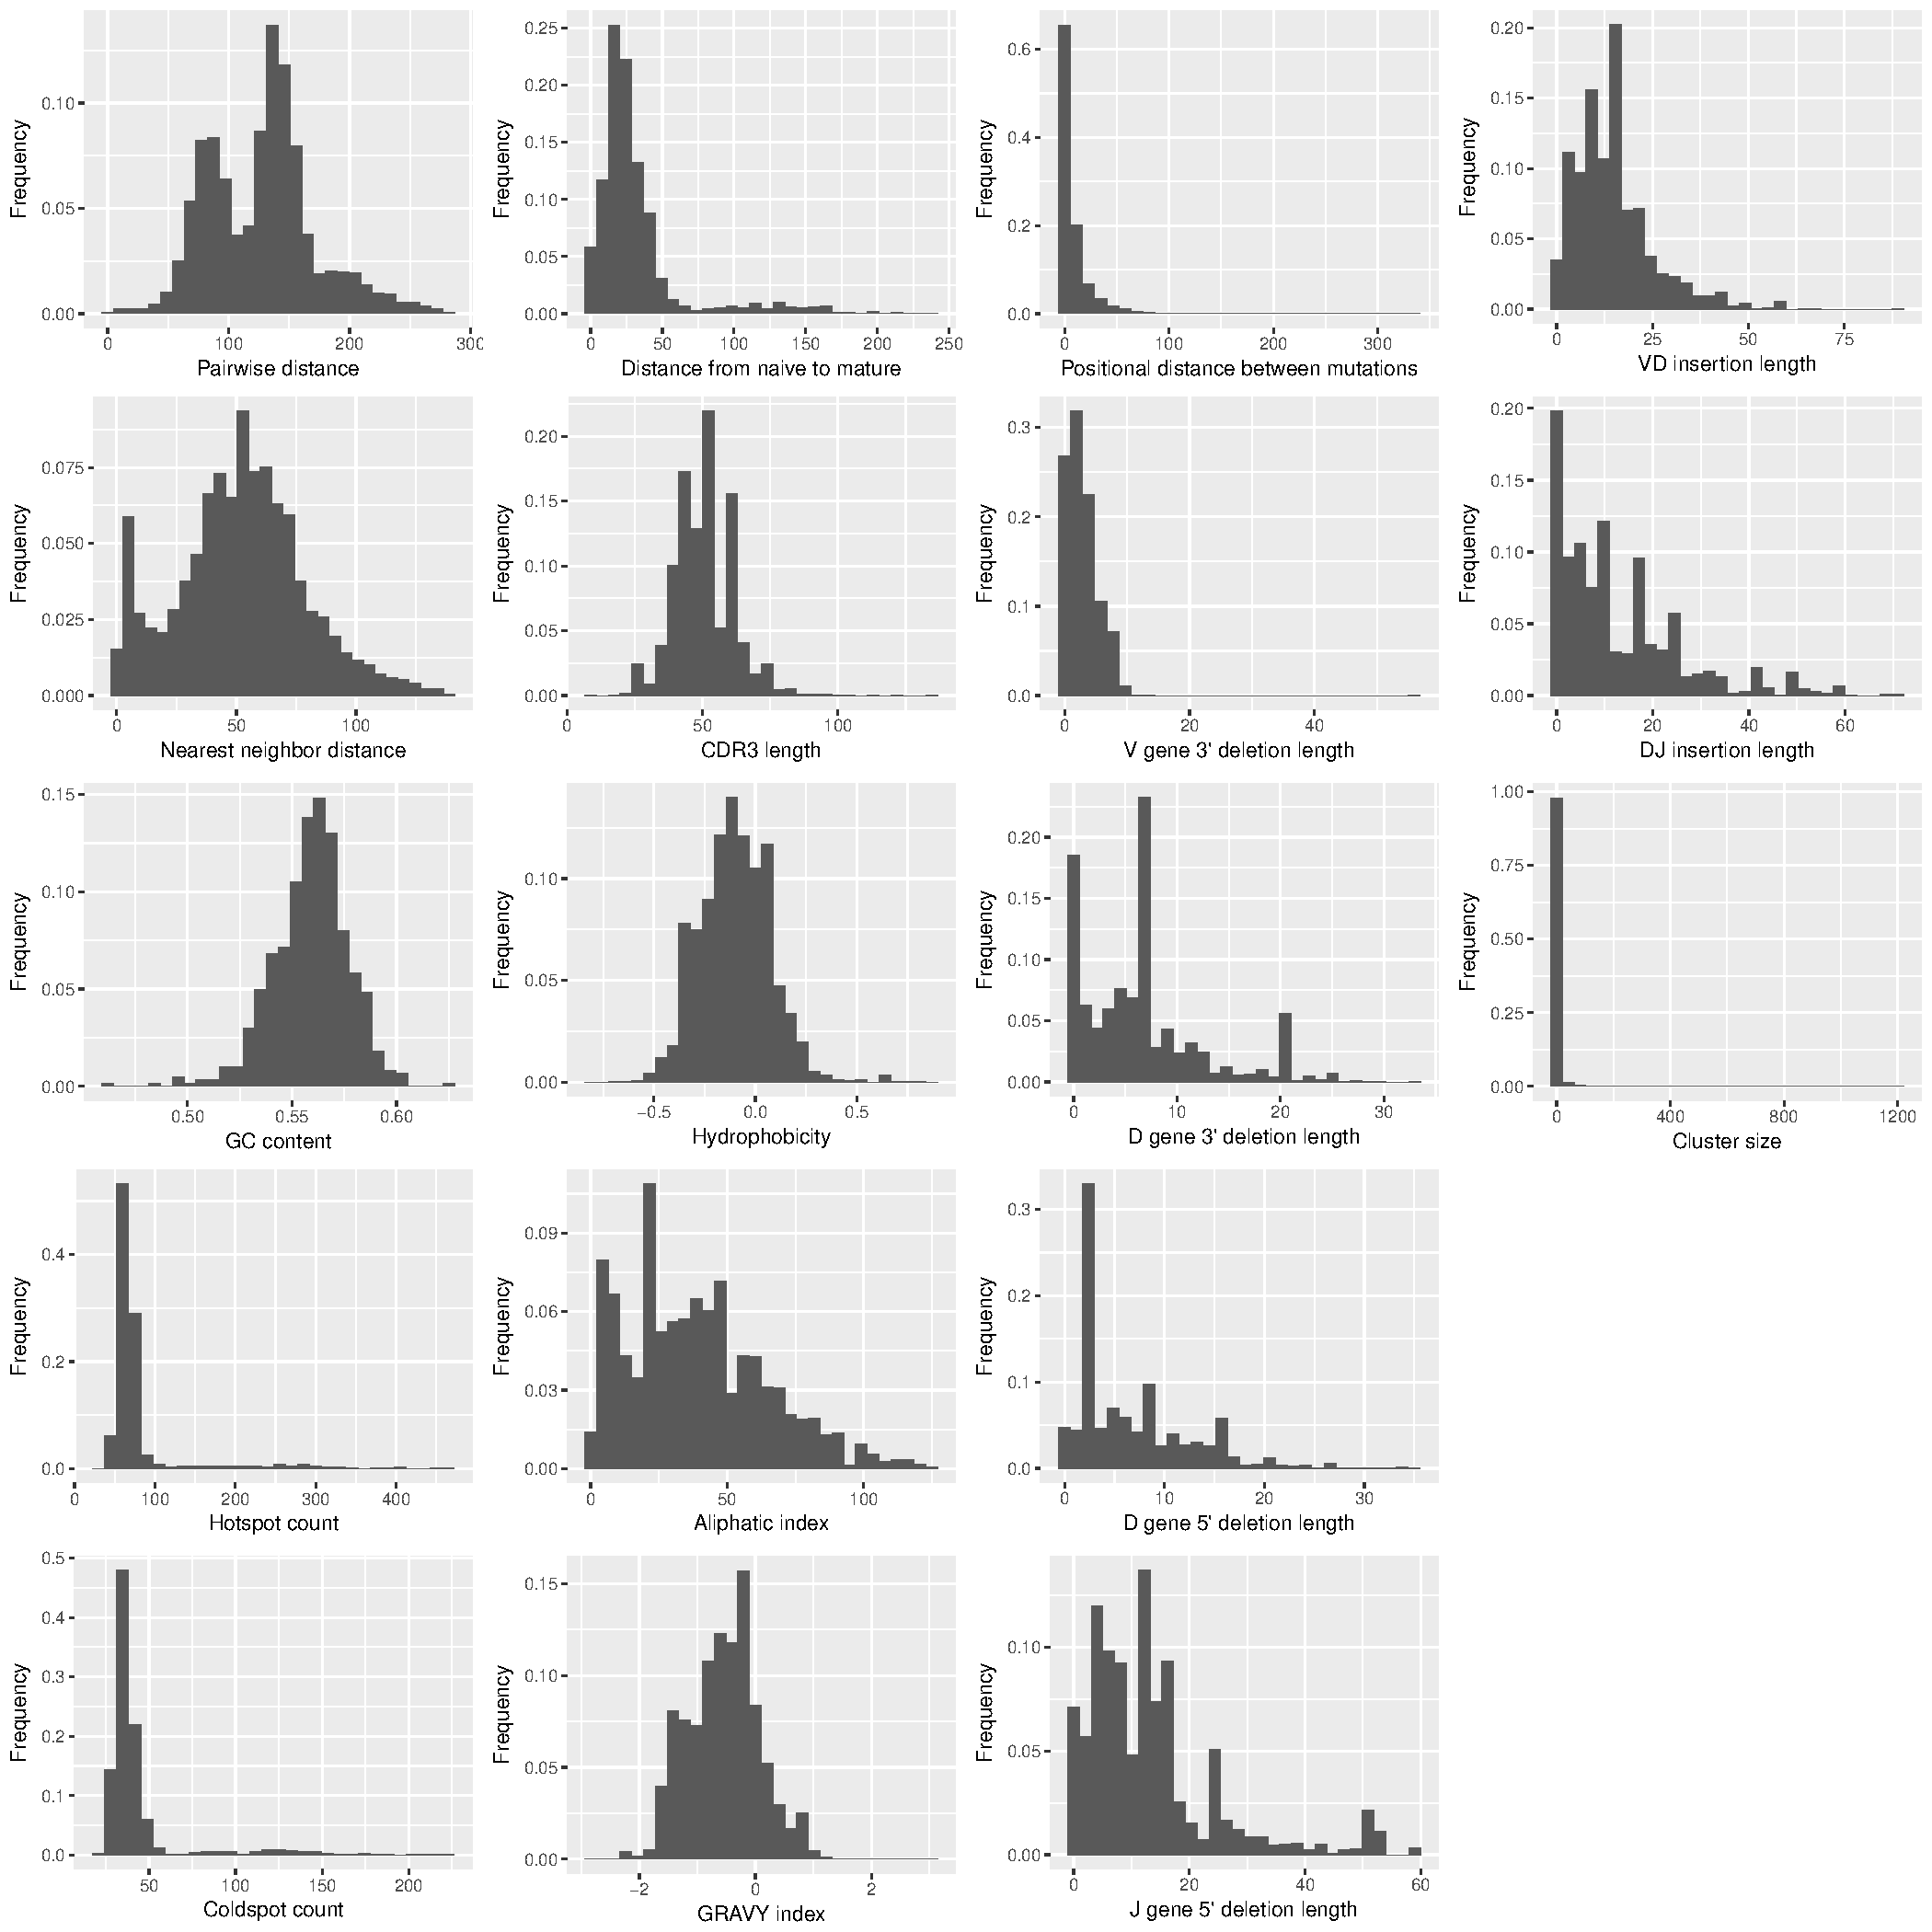
\includegraphics[width=0.75\linewidth]{Images/master_plot.pdf}
\end{center}
\end{frame}

\begin{frame}\frametitle{Univariate distribution plots for 2 datasets}
\begin{center}
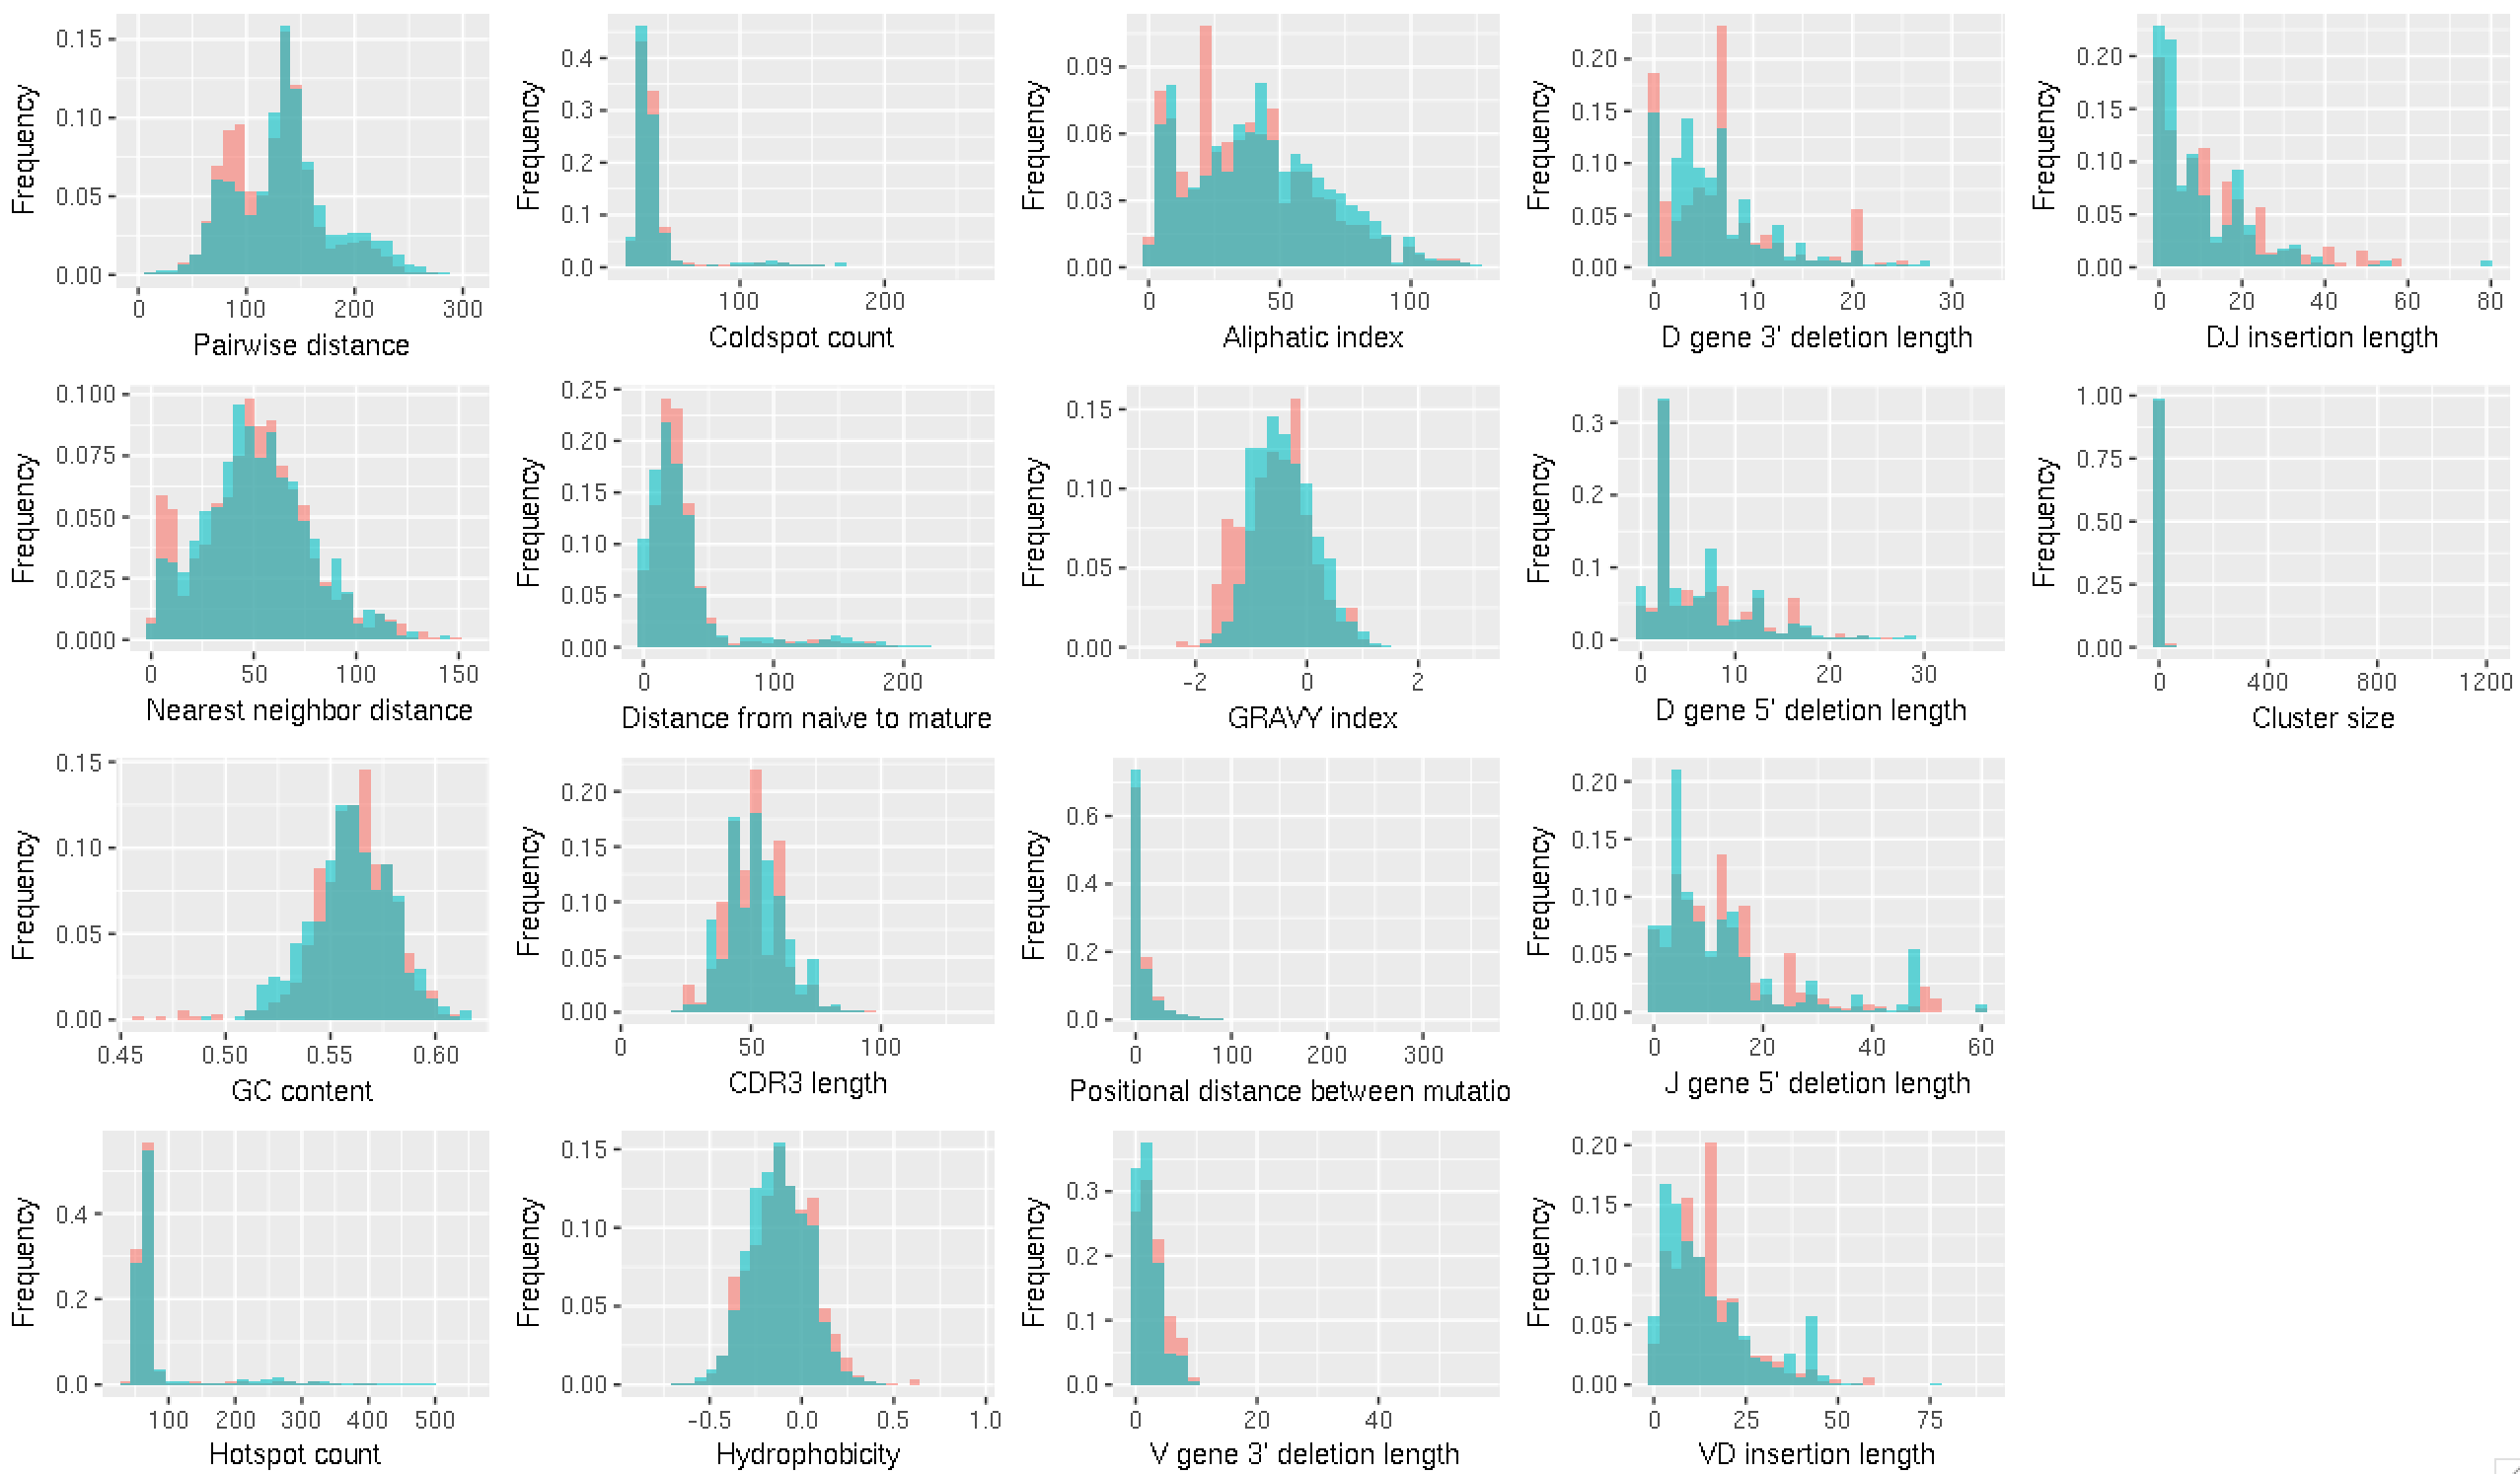
\includegraphics[width=\linewidth]{Images/Dual_summaries.png}
\end{center}
\end{frame}

\section{Automatic distribution subsampling}

\begin{frame}\frametitle{Sampling distributions}
\begin{itemize}
\item Some useful summaries are \emph{really} slow to compute
\begin{itemize}
\item distance-based
\medskip
\item hot- and coldspot counts
\end{itemize}
\bigskip
\item For distributional summaries, we don't need the exact distribution, just the behavior
\bigskip
\item
But, taking one subsample usually doesn't cut it
\bigskip
\item Let's subsample in a principled way
\end{itemize}
\end{frame}

\begin{frame}\frametitle{Example: pairwise distance distribution}
\begin{itemize}
\item
Computing the pairwise distance distribution of $n$ sequences grows very quickly with $n$
\bigskip
\item
If we have a repertoire of $n = 50,000$ sequences, we could try to subsample $k = 10,000$ and call it good. But this will still be very slow. 
\item
Even $k = 1,000$ takes some time, and we're not sure how much we're losing.

\bigskip
\item But, computing this distribution for $k = 100$ is cake. 
\end{itemize}
\end{frame}

\begin{frame}\frametitle{Example: pairwise distance distribution}
\begin{itemize}
\item Idea:
\begin{itemize}
\item
Compute the pairwise distance distribution of a small subsample ($k = 100$)
\item
Append this to a rolling distribution
\item
Stop when successive iterates stop changing
\end{itemize}
\item
Here, an iterate is a distribution (i.e., a vector of integers)
\bigskip
\item
Consider converged if the JS divergence between successive iterates is less than some tolerance $\eps$
\end{itemize}
\end{frame}

\begin{frame}\frametitle{Performance by tolerance}
\begin{center}
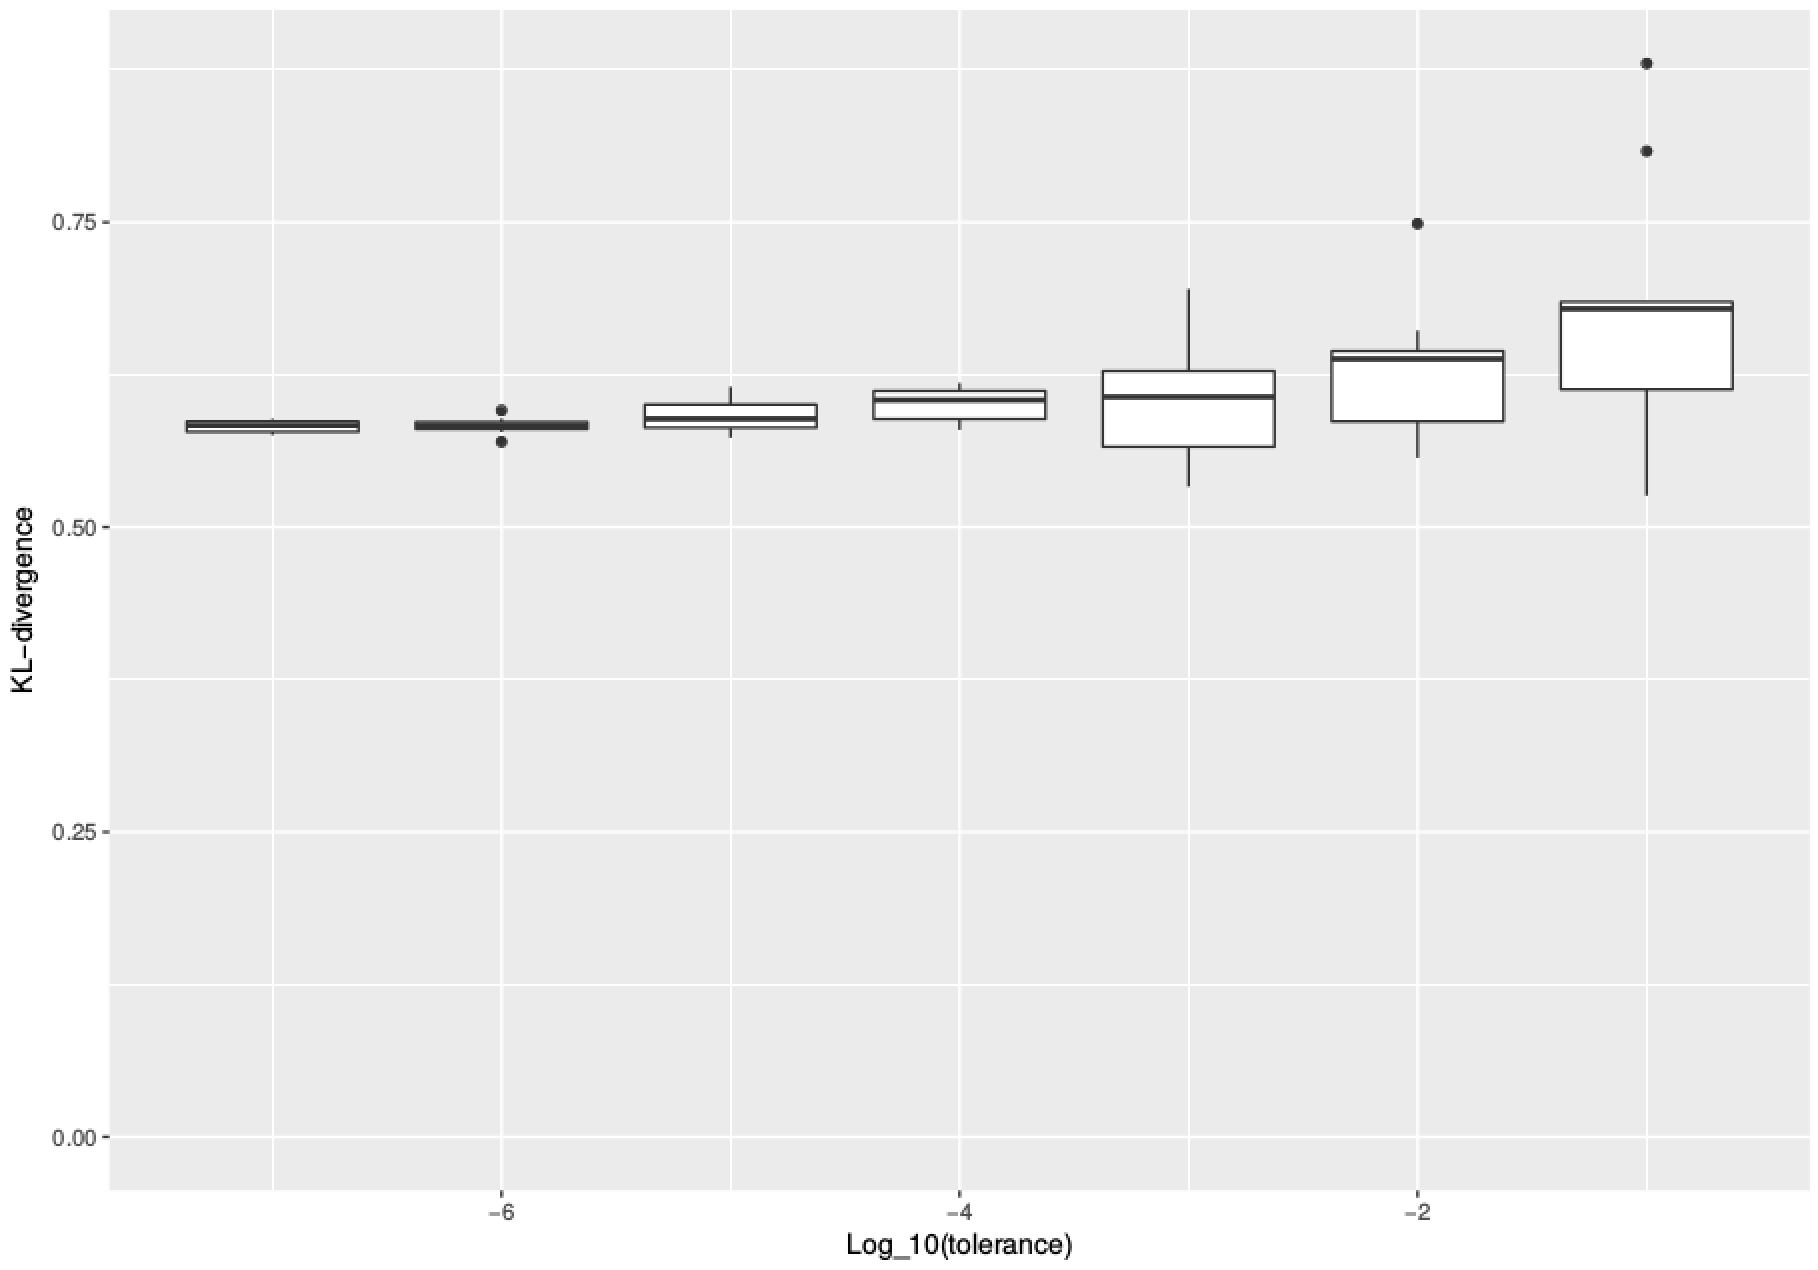
\includegraphics[width=\linewidth]{/Users/brandenolson/Code/Matsen/Manuscripts/sumrep-ms/Figures/PairwiseDistance/div_by_tol.pdf}
\end{center}
\end{frame}

\begin{frame}\frametitle{Performance by size of full dataset}
\begin{center}
\includegraphics[width=\linewidth]{/Users/brandenolson/Code/Matsen/Manuscripts/sumrep-ms/Figures/PairwiseDistance/div_by_size_and_tol.pdf}
\end{center}
\end{frame}

\begin{frame}\frametitle{Performance by summary statistic}

\end{frame}

\begin{frame}
\begin{center}
\Huge
Questions?
\end{center}
\end{frame}

\end{document}























